\documentclass[border=10pt,tikz]{standalone}
\usepackage{tikz}
\usetikzlibrary{shapes,arrows,positioning,calc}

\begin{document}

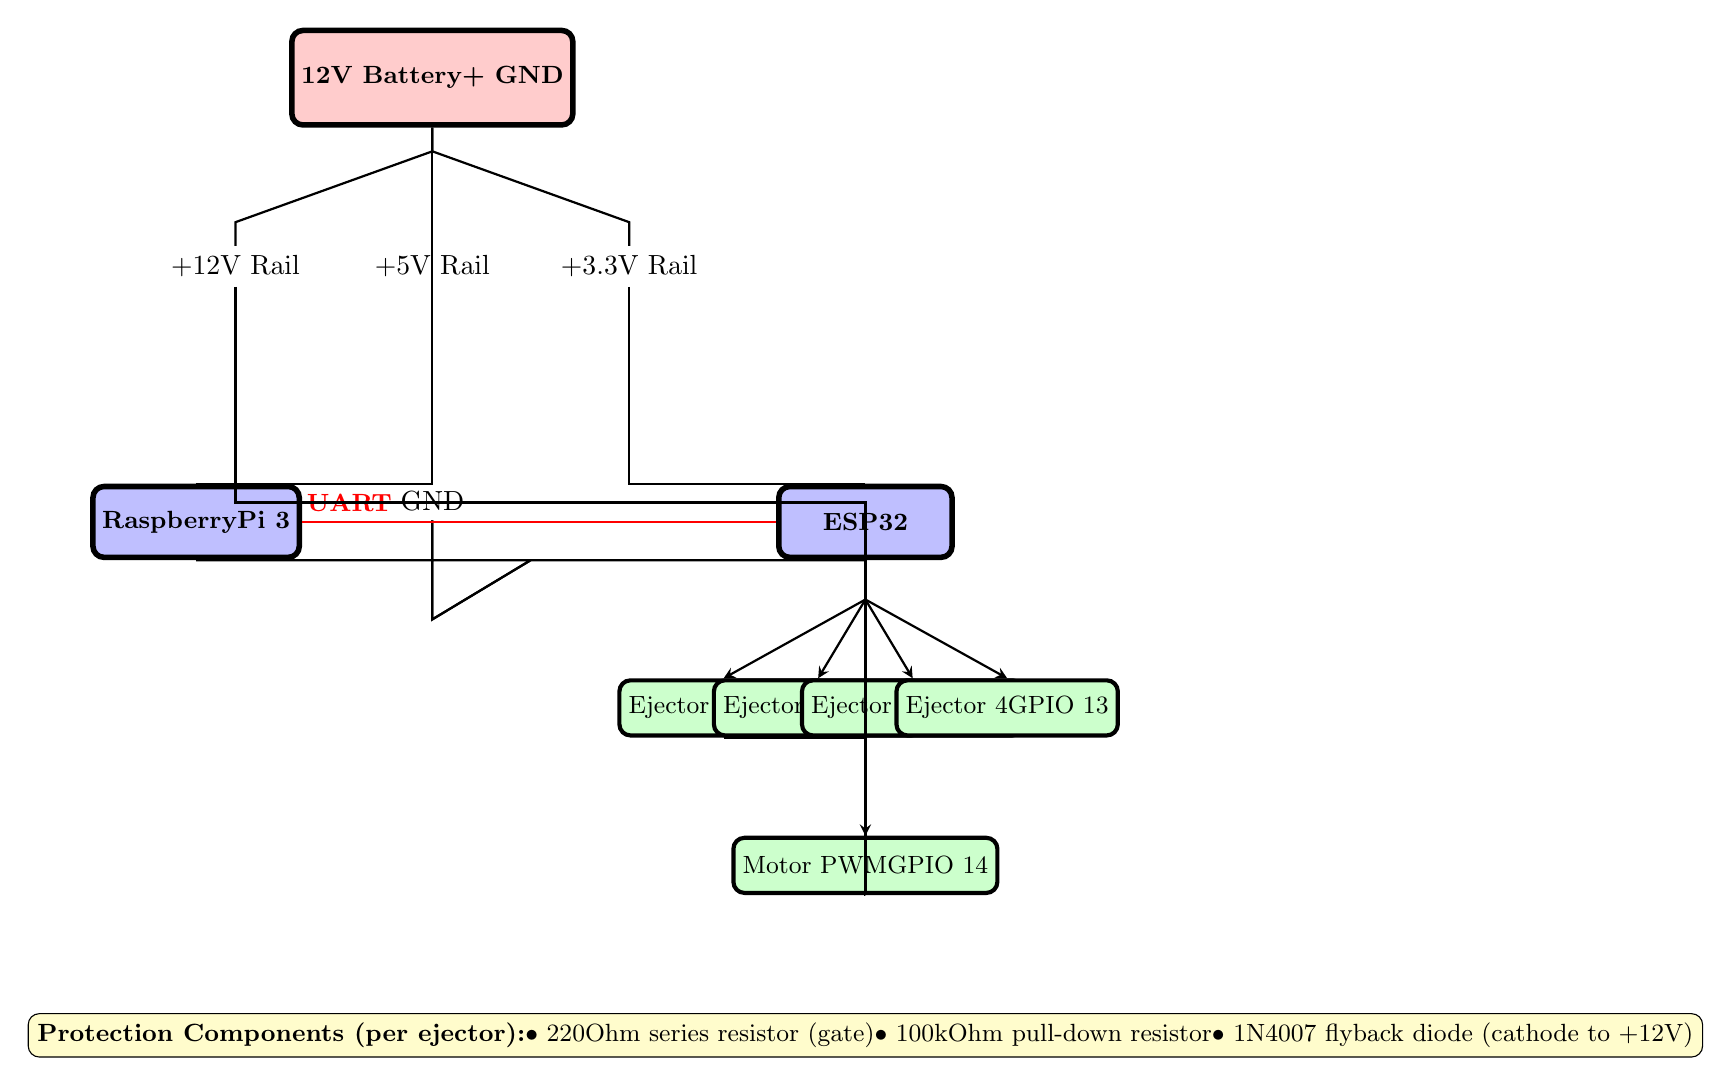
\begin{tikzpicture}[node distance=2cm, auto]

% Define styles
\tikzstyle{battery} = [rectangle, rounded corners, minimum width=2cm, minimum height=1.2cm, text centered, draw=black, fill=red!20, line width=2pt, font=\small\bfseries]
\tikzstyle{processor} = [rectangle, rounded corners, minimum width=2.2cm, minimum height=0.9cm, text centered, draw=black, fill=blue!25, line width=2pt, font=\small\bfseries]
\tikzstyle{device} = [rectangle, rounded corners, minimum width=1.8cm, minimum height=0.7cm, text centered, draw=black, fill=green!20, line width=1.5pt, font=\small]
\tikzstyle{connection} = [circle, minimum size=0.15cm, draw=black, fill=black]
\tikzstyle{arrow} = [thick, ->, >=stealth]
\tikzstyle{line} = [thick, draw=black]

% Power Supply
\node (battery) [battery] {12V Battery\\+ GND};

% Distribution rails
\node (rail_12v) [below=1.5cm of battery, xshift=-2.5cm] {+12V Rail};
\node (rail_5v) [below=1.5cm of battery, xshift=0cm] {+5V Rail};
\node (rail_3v3) [below=1.5cm of battery, xshift=2.5cm] {+3.3V Rail};
\node (rail_gnd) [below=4.5cm of battery] {GND};

% Connections from battery to rails
\draw [line] (battery.south) -- ++(0, -0.3) -- ++(-2.5, -0.9) -- (rail_12v.north);
\draw [line] (battery.south) -- ++(0, -0.3) -- (rail_5v.north);
\draw [line] (battery.south) -- ++(0, -0.3) -- ++(2.5, -0.9) -- (rail_3v3.north);
\draw [line] (battery.south) |- (rail_gnd.north);

% Processors
\node (pi) [processor, below=2.5cm of rail_5v, xshift=-3cm] {Raspberry\\Pi 3};
\node (esp) [processor, below=2.5cm of rail_3v3, xshift=3cm] {ESP32};

% Connect to power
\draw [line] (rail_5v) |- (pi.north);
\draw [line] (rail_3v3) |- (esp.north);
\draw [line] (rail_gnd) |- ++(0, -1.5) -- ($(pi.south)!0.5!(esp.south)$) -- (pi.south);
\draw [line] (rail_gnd) |- ++(0, -1.5) -- ($(pi.south)!0.5!(esp.south)$) -- (esp.south);

% UART Connection
\draw [line, color=red] (pi.east) -- ++(1.2, 0) node[midway, above, color=red, font=\small\bfseries] {UART} -- (esp.west);

% Output devices from ESP32
\node (ejector1) [device, below=1.5cm of esp, xshift=-1.8cm] {Ejector 1\\GPIO 4};
\node (ejector2) [device, below=1.5cm of esp, xshift=-0.6cm] {Ejector 2\\GPIO 5};
\node (ejector3) [device, below=1.5cm of esp, xshift=0.6cm] {Ejector 3\\GPIO 12};
\node (ejector4) [device, below=1.5cm of esp, xshift=1.8cm] {Ejector 4\\GPIO 13};
\node (motor) [device, below=3.5cm of esp] {Motor PWM\\GPIO 14};

% Connect ESP32 to outputs
\draw [arrow] (esp.south) -- ++(0, -0.5) -- (ejector1.north);
\draw [arrow] (esp.south) -- ++(0, -0.5) -- (ejector2.north);
\draw [arrow] (esp.south) -- ++(0, -0.5) -- (ejector3.north);
\draw [arrow] (esp.south) -- ++(0, -0.5) -- (ejector4.north);
\draw [arrow] (esp.south) -- ++(0, -0.5) -- (motor.north);

% Power distribution to outputs
\draw [line] (rail_12v) -- ++(0, -3) -| ($(ejector1.south)!0.5!(ejector4.south)$) |- (ejector1.south);
\draw [line] (rail_12v) -- ++(0, -3) -| ($(ejector1.south)!0.5!(ejector4.south)$) |- (motor.south);

% Add legend/notes
\node [draw=black, fill=yellow!20, rounded corners, minimum width=6cm, below=0.5cm of motor, yshift=-1cm, font=\small] {
\textbf{Protection Components (per ejector):} \\
$\bullet$ 220Ohm series resistor (gate) \\
$\bullet$ 100kOhm pull-down resistor \\
$\bullet$ 1N4007 flyback diode (cathode to +12V)
};

\end{tikzpicture}

\end{document}
